\documentclass[compress]{beamer}

\mode<presentation>
\usetheme{Singapore}
\usecolortheme{rose}

% \usepackage{amsmath,amsfonts,amssymb}
% \usepackage{colortbl}
% \usepackage{hyperref}
\usepackage{tikz}
\usetikzlibrary{calc}
\usetikzlibrary{positioning}
\usetikzlibrary{calc,intersections,through,backgrounds}

%%% Template Setting

%% Font
\usefonttheme[onlylarge]{structuresmallcapsserif}
\usefonttheme[onlysmall]{structurebold}
\setbeamerfont{title}{shape=\itshape,family=\rmfamily}
\setbeamertemplate{frametitle}[default][center]


\title{Molding CNNs for text: non-linear, non-consecutive convolutions}
\author{Tao Lei, Regina Barzilay, and Tommi Jaakkola}
\institute{Presented by Shih-Ming Wang \\ NLPLab, Institute of Information Science, Academia Sinica}
\date{07-5-2016}
\subject{Computer Science}

\graphicspath{{img/}}

\begin{document}
\beamertemplatenavigationsymbolsempty

\begin{frame}
 \maketitle
\end{frame}

\begin{frame}
 \frametitle{Outline}
 \tableofcontents
\end{frame}

\section{Introduction}
    \begin{frame}{\secname}
        \begin{block}{Motivation}
            \begin{itemize}
                \item Deep learning \& Convolution neural network (CNN) have led to success in many NLP problems
                \item Convolution operation is a \textbf{linear} mapping over \textbf{n-gram} vectors
                \item Target: \textbf{non-linear} operation over \textbf{non-consecutive} n-grams (e.g., ``\underline{not} that \underline{good}'')
            \end{itemize}
            
        \end{block}
    \end{frame}

\section{Background}
    \begin{frame}{\secname}
        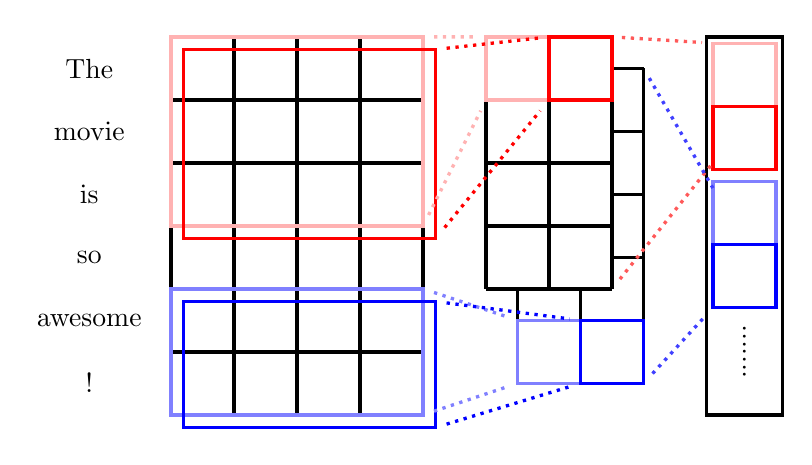
\begin{tikzpicture}
            [scale=0.8,
            border/.style={very thick},
            link/.style={very thick, dotted},
            ]
            \colorlet{f1color}{red!30!white}
            \colorlet{f2color}{red}
            \colorlet{f3color}{blue!50!white}
            \colorlet{f4color}{blue}
            \begin{scope}[shift={(0,0)}]
                % words
                \begin{scope}[shift={(-1.3,.5)}]
                    \node at (0,5) {The};
                    \node at (0,4) {movie};
                    \node at (0,3) {is};
                    \node at (0,2) {so};
                    \node at (0,1) {awesome};
                    \node at (0,0) {!};
                \end{scope}

                \begin{scope}[shift={(0, 6)}]
                    \draw[border, step=1cm] (0,-6) grid (4, 0);
                    % f1
                    \draw[border, f1color] (0,0) rectangle +(4, -3) node(A1){} +(4,0) node(A2){};
                    % f2
                    \draw[border, f2color] (.2,-.2) rectangle +(4, -3) node (B1){} +(4,0) node(B2){};
                \end{scope}

                \begin{scope}[shift={(0, 2)}]
                    % f3
                    \draw[border, f3color] (0,0) rectangle +(4,-2) node(C1){} +(4,0) node(C2){}; 
                    % f4
                    \draw[border, f4color] (.2,-.2) rectangle +(4,-2) node(D1){} +(4,0) node(D2){}; 
                \end{scope}

                \begin{scope}[shift={(5, 6)}]
                    \begin{scope}[shift={(.5,-.5)}]
                        \draw[border, step=1cm] (0,-5) grid (2,0);
                        \draw (2,0) node(F1){} (2,-5) node(F2){};
                        \begin{scope}[shift={(0,-4)}]
                            % f3_2
                            \draw[border, f3color] (0,0) node(C4){} rectangle +(1,-1) +(0,-1)node(C3){};
                            \draw[border, f4color] (1,0) node(D4){} rectangle +(1,-1)  +(0,-1)node(D3){};
                        \end{scope}
                        \fill[white] (-.1,.1) rectangle (1.5,.-3.5);
                    \end{scope}

                    \draw[border, step=1cm] (0,-4) grid (2,0);
                    \draw (2,0) node(E1){} (2,-4) node(E2){};
                    % f1_2
                    \draw[border, f1color] (0,0) node(A4){} rectangle +(1,-1) +(0,-1)node(A3){};
                    % f2_2
                    \draw[border, f2color] (1,0) node(B4){} rectangle +(1,-1)  +(0,-1)node(B3){};
                \end{scope}

                \begin{scope}[shift={(8.5, 6)}]
                    \draw[border] (0,0) rectangle (1.2,-6);
                    \begin{scope}[shift={(.1, -.1)}]
                        \draw[f1color, border] (0,0) node(E3){} rectangle +(1,-1);
                        \draw[f2color, border] (0,-1) rectangle +(1,-1) +(0,-1) node(E4){};
                    \end{scope}

                    \begin{scope}[shift={(.1, -2.3)}]
                        \draw[f3color, border] (0,0) node(F3){} rectangle +(1,-1);
                        \draw[f4color, border] (0,-1) rectangle +(1,-1) +(0,-1) node(F4){};
                    \end{scope}
                    \draw ++(.6,-5 ) node[rotate=90] {.......};
                \end{scope}

                \draw[link, f1color] (A1) -- (A3);
                \draw[link, f1color] (A2) -- (A4);
                \draw[link, f2color] (B1) -- (B3);
                \draw[link, f2color] (B2) -- (B4);
                \draw[link, f3color] (C1) -- (C3);
                \draw[link, f3color] (C2) -- (C4);
                \draw[link, f4color] (D1) -- (D3);
                \draw[link, f4color] (D2) -- (D4);

                \draw[link, f1color!50!f2color] (E1) -- (E3);
                \draw[link, f1color!50!f2color] (E2) -- ($(E4)+(0,0.1)$);
                \draw[link, f3color!50!f4color] (F1) -- ($(F3)+(0,-0.1)$);
                \draw[link, f3color!50!f4color] (F2) -- (F4);  
            \end{scope}
        \end{tikzpicture}
    \end{frame}

\section{Model Description}
    \subsection{Tensor-based Feature Mapping}
        \begin{frame}[allowframebreaks]{\subsecname}
            \begin{block}{Outer product}
                \begin{itemize}
                    \item Use outer product operation instead of linear combination
                    \item Consider bi-gram $(x_1, x_2)$ (row vectors) as example:
                \end{itemize}
                \begin{table}[t]
                    \centering
                    \begin{tabular}{lrrr}
                                & Linear             & Outer Product        & 3D case                             \\ \hline
                    Raw         & $[x_1; x_2]$       & $x_1^T \cdot x_2$    & $x_1 \bigotimes x_2 \bigotimes x_3$ \\ \hline
                    Dim(raw)    & $2\times d$        & $d\times d$          & $d\times d \times d$                \\ \hline
                    Dim(Kernel) & $h\times2\times d$ & $h\times d \times d$ & $h\times d \times d \times d$       \\ \hline
                    Output      & $h\times 1$        & $h \times 1$         & $h \times 1$
                    \end{tabular}
                \end{table}
                ,where $(x_1 \bigotimes x_2 \bigotimes x_3)_{ijk} = x_{1i} \cdot x_{2j} \cdot x_{3k}$
            \end{block}
        \framebreak
            \begin{block}{Parameter Explosion}
                \begin{itemize}
                    \item Kernel $T$ has $h\times d^n$ parameters for n-gram
                    \item Solution: Decompose $T$ in to sum of $\bar{h}$ rank-1 tensors
                    \begin{table}[t]
                    \centering
                    \begin{tabular}{lll}
                            & 2D                                                              & 3D
                           \\ \hline
                    Dim(T)  & $h\times d \times d$                                            & $h\times d \times d \times d$                                                  \\ \hline
                    T'      & $\sum\limits_{i=1}^{\bar{h}} O_i \bigotimes P_i \bigotimes Q_i$ & $\sum\limits_{i=1}^{\bar{h}} O_i \bigotimes P_i \bigotimes Q_i \bigotimes R_i$ \\ \hline
                    \end{tabular}
                    \end{table}
                    ,where\\
                    $O \in \mathbb{R}^{\bar{h} \times h}$; $P, Q, R \in \mathbb{R}^{h\times d}$; \\
                    $O_i \in \mathbb{R}^h$; $P_i, Q_i, R_i \in \mathbb{R}^d$

                    For simplity, $\bar{h}=h$.
                \end{itemize}
            \end{block}
        \framebreak
            \begin{block}{Feature Map Calculation}
                \begin{table}[t]
                \centering
                \begin{tabular}{lll}
                        & 2D                                                              & 3D                                                                             \\ \hline
                Feature & $x_1 \bigotimes x_2$                                            & $x_1 \bigotimes x_2 \bigotimes x_3$                                            \\ \hline
                Kernel  & $\sum\limits_{i=1}^{\bar{h}} O_i \bigotimes P_i \bigotimes Q_i$ & $\sum\limits_{i=1}^{\bar{h}} O_i \bigotimes P_i \bigotimes Q_i \bigotimes R_i$ \\ \hline
                Output  & $O \cdot (Px_1 \bigodot Qx_2)$                                   & $O \cdot (Px_1 \bigodot Qx_2 \bigodot Rx_3)$
                \end{tabular}
                \end{table}
                ,where $\bigodot$ is element-wise product. \\
                \begin{itemize}
                    \item $Px_1$ is a linear transformation of $x_1$
                    \item Higher-order terms (i.e. $x_1 \bigotimes x_2 \bigotimes x_3$) arise from the element-wise products.
                \end{itemize}
            \end{block}
        \end{frame}
    \subsection{Non-consecutive n-gram Features}
        \begin{frame}[allowframebreaks]{\subsecname}
            \begin{block}{Non-consecutive n-gram}
                \begin{itemize}
                    \item Example: ``\underline{not} nearly as \underline{good}'' 
                    \item Intuition: consider all words previous to current word, with decay.
                \end{itemize}
            \end{block}
        \framebreak
            \begin{block}{Calculation of non-consecutive n-gram}
                \begin{itemize}
                    \item Let $z[i,j,k] \in \mathbb{R}^h$ denote the feature corresponding to the 3-gram $(x_i, x_j, x_k)$ 
                    \item $z[i,j,k] = O(Px_i \bigodot Qx_j \bigodot Rx_k)$
                    \item Define the \textbf{aggregate representation} $z_3[k]$ as a weighted sum of all $z[i,j,k], i<j<k$
                    \item $z_3[k] = \sum\limits_{i<j<k}z[i,j,k] \times \lambda^{(k-j-1)+(j-i-1)}$
                    \item $\lambda \rightarrow 0$, the model degrades to traditional 3-gram
                    \item Comment: somehow extends effective window size. 
                \end{itemize}
            \end{block}
                \framebreak
            \begin{block}{Dynamic Programming}
                \begin{itemize}
                    \item Calculating all $z_3[k]$ is $O(L^3)$
                    \item In practice, it is calculated as follows:
                    \begin{equation*}
                        \begin{aligned}
                            & z_1[k] = Px_i \\
                            & s_1[k] = \lambda \cdot s_1[k-1] + f_1[k] \\
                            & z_2[k] = s_1[k-1] \bigodot Qx_k \\
                            & s_2[k] = \lambda \cdot s_2[k-1] + f_2[k]\\
                            & z_3[k] = s_2[k-1] \cdot Rx_k \\
                            & z[k]=O(z_1[k]+z_2[k]+z_3[k])
                        \end{aligned}
                    \end{equation*}
                    \item Use summation of uni-gram, bi-gram, and tri-gram instead of only tri-gram  
                \end{itemize}
            \end{block}
        \end{frame}
    \subsection{Overall Architecture}
        \begin{frame}{\subsecname}
      		\includegraphics[width=\textwidth]{molding_cnn.png}
        \end{frame}
        
        % \begin{frame}{\subsecname}
      	% 	\includegraphics[width=\textwidth]{img/molding_cnn.png}
        % \end{frame}

\section{Experiments}
\begin{frame}[allowframebreaks]{\secname}
    \begin{block}{Task}
        \begin{itemize}
            \item Sentiment classification 
                \begin{itemize}
                    \item Stanford Sentiment Treebank
                    \item Binary (6920/872/1821) \& Fine-grained (5 class) (8544/1101/2210). 
                \end{itemize}
            \item Chinese news categorization
                \begin{itemize}
                    \item Sogou Chinese news corpora
                    \item 10 news categories (79520/9940/9940)
                \end{itemize}
        \end{itemize}
    \end{block}
    \framebreak
        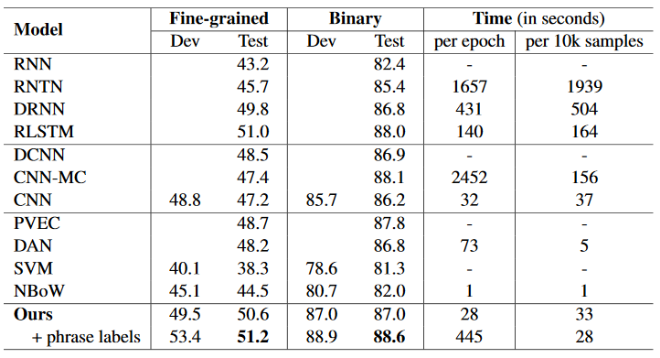
\includegraphics[width=\textwidth]{performance.png}
\end{frame}

\section{Error Analysis}
    \begin{frame}{\secname\ I}
        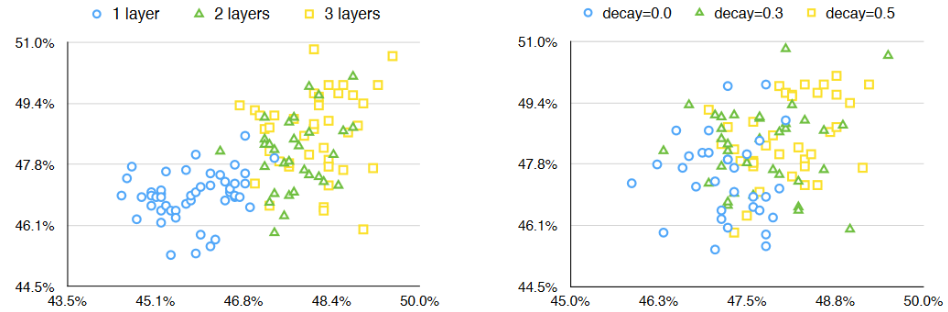
\includegraphics[width=\textwidth]{error_analysis.png}
    \end{frame}
    \begin{frame}{\secname\ II}
        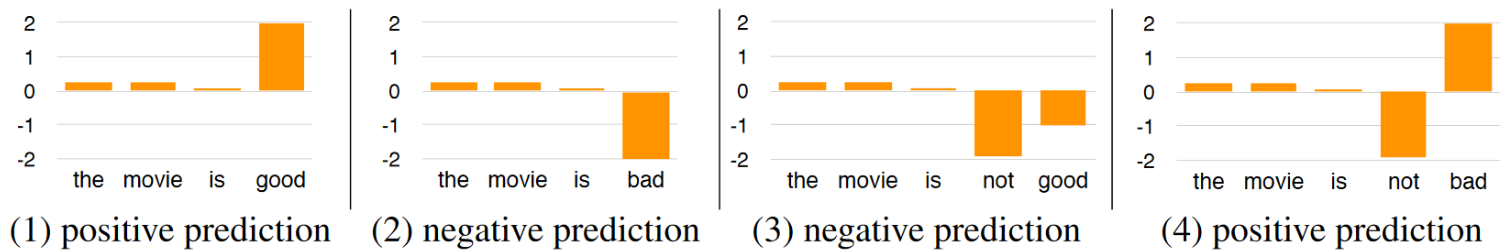
\includegraphics[width=\textwidth]{error_analysis2.png}
    \end{frame}

\section{Conclusion}
    \begin{frame}{\secname}
        \begin{itemize}
            \item A feature mapping operator for CNN is proposed
            \item The method considers non-linear interaction within n-gram
            \item Non-consecutive n-gram is considered with a weighted sum over previous n-gram
            \item The method is memory-efficient by factorizing kernel tensor
            \item The method is time-efficient by adopting dynamic programming
            \item It achieves state-of-the-art performance
        \end{itemize}
    \end{frame}

\end{document}
